\section*{Exercícios Extra}

\begin{enumerate}[label=E\arabic*]

%%%%%%%%%%%%%%%%%%%%%%%%%%%%%%%%%%%%%%%%%%%%%%%%%%%%%%%%%%%%%%%

\item \textbf{Inferência Bayesiana sequencial} \par
Motivado pela Figura 2.3 do livro, reproduza o
experimento da jogada de moeda considerando que foram realizadas 5 jogadas e que a
probabilidade de se obter cara é dada por `$\mu = 0,7$'. Plote a distribuição a priori e todas
as 5 distribuições a posteriori geradas ao longo do processo iterativo. Considere que a
distribuição a priori é uma Beta com parâmetros `$a$' e `$b$' escolhidos da seguinte forma:

1º caso: $a = b = 1$

2º caso: $a = b = 2$

Compare os resultados obtidos nos 2 casos.

OBS: Para uma comparação justa entre os 2 casos, primeiro gere os 5 dados (saídas do
experimento da moeda, amostrados da Bernoulli definida no enunciado) e depois aplique
o aprendizado sequencial para os 2 casos (i.e., para ambas as prioris) usando
exatamente os mesmos dados gerados.
\begin{figure}[H]
    \caption{\textbf{Figura 2.3 do Bishop}}
       \centering
       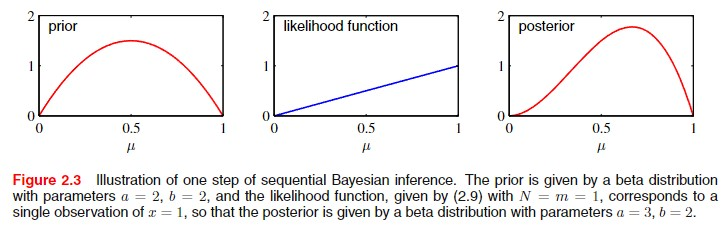
\includegraphics{bishop_23.jpg}
\end{figure}
\par
\textbf{Solução:}

De forma a atender a este exercício foi implementado em python uma função que recebe como entrada uma amostra com 5 dados, a qual é gerada por uma distribuição de Bernoulli com $\mu=0.7$, e uma lista com dois valores para os parâmetros $a$ e $b$ (um para cada caso pedido). Para cada par $(a_0,b_0)$ a função calcula a priori fazendo Beta$(\mu|a_0,b_0)$ e depois começa a fazer iterações para cada dado da amostra. A cada iteração os valores de $a$ e $b$ são atualizados por 
\begin{equation*}
    a_N = a_0 + m \quad \text{e}
\end{equation*}
\begin{equation*}
    b_N = b_0 + (N - m),
\end{equation*}
onde $N$ é o tamanho da amostra até aquela iteração e $m$ é a quantidade de sucessos (caras) até ali. A likelihood é calculada por 
\begin{equation*}
    \prod_{n=1}^{N}\mu^{x_n}(1-\mu)^{(1-x_n)}
\end{equation*}
e a posteriori calcula por Beta$(\mu|a_N,b_N)$. No final são plotados a priori, as 5 likelihoods e as 5 posterioris calculadas. O resultado pode ser observado na figura abaixo.

\begin{figure}[H]
    \caption{\textbf{Plot do resultado}}
       \centering
       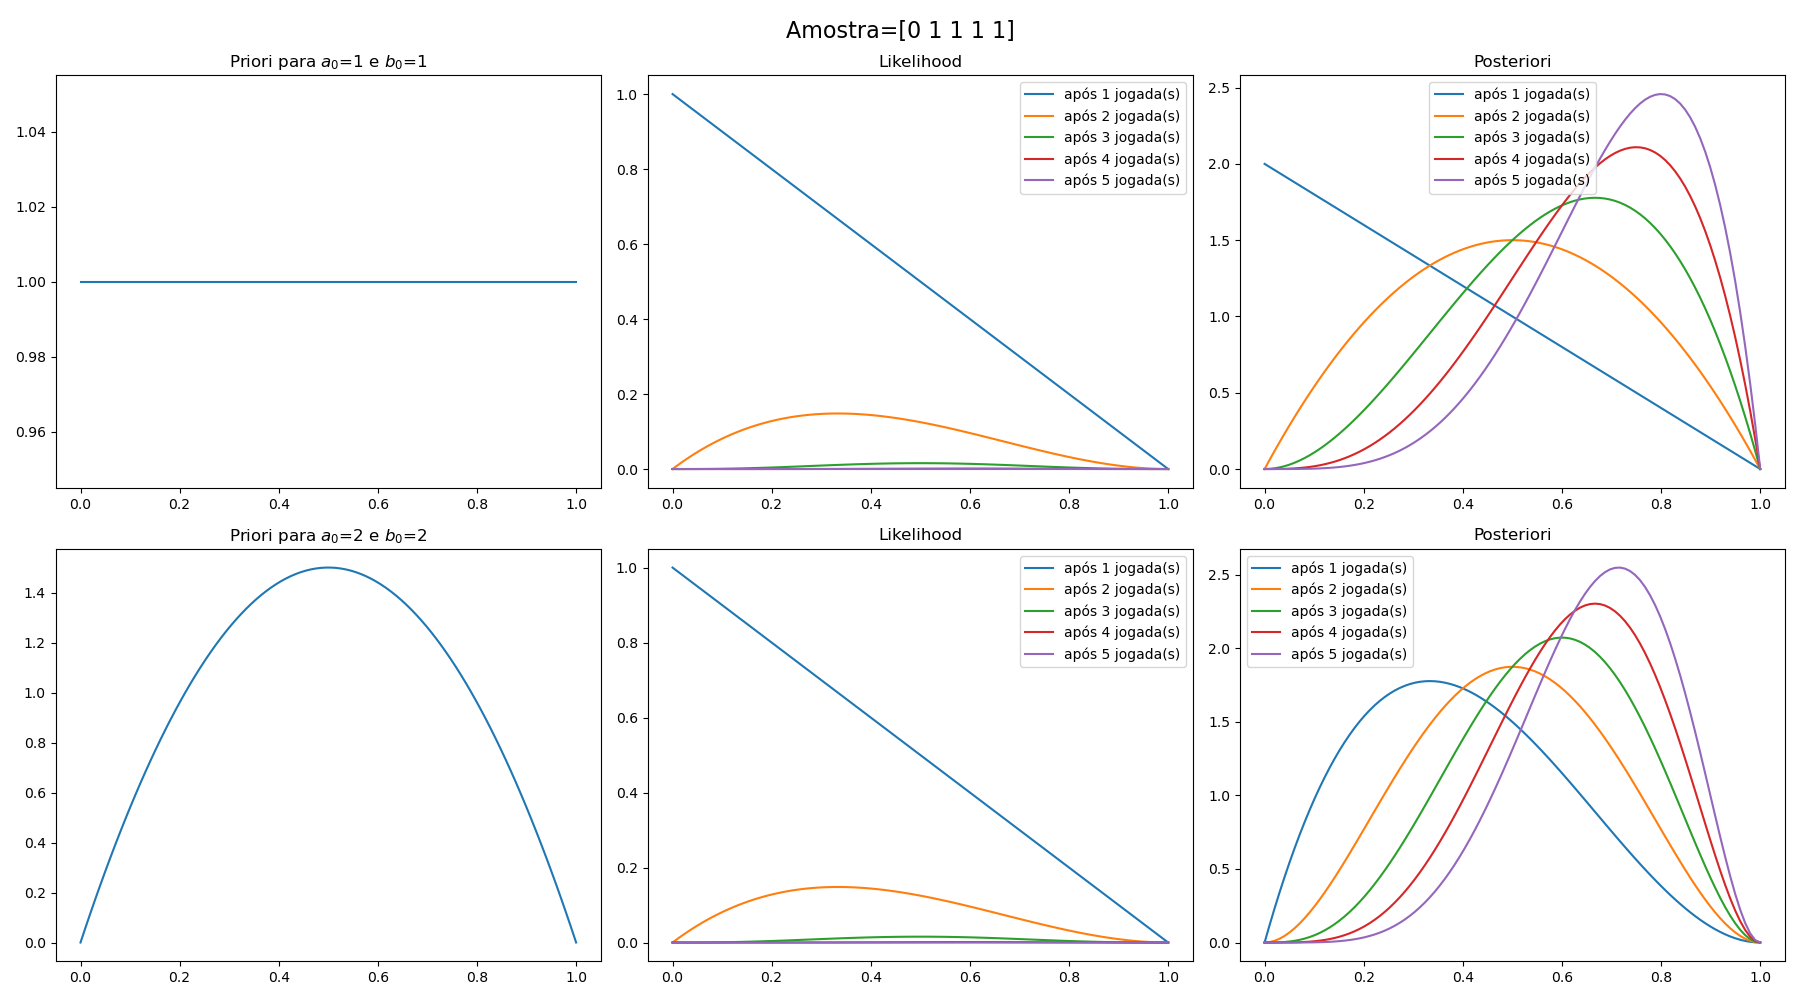
\includegraphics[width=\textwidth]{ex1.png}
\end{figure}

É possível observar como a inferência bayesiana sequencial ajusta a distribuição de probabilidade à medida que novas observações são feitas, atualizando continuamente a distribuição posteriori com base nos novos dados.

A diferença na inicialização da priori com $a = b = 1$ e $a = b = 2$ impacta a sensibilidade da distribuição posteriori aos dados observados. Com $a = b = 1$, a priori é uniforme, implicando que todos os valores de $\mu$ são igualmente prováveis inicialmente, tornando a posteriori altamente responsiva aos dados. Já com $a = b = 2$, a priori é mais concentrada em torno de 0.5, refletindo uma crença inicial de que a probabilidade de sucesso é 50\% (moeda justa), resultando em uma posteriori mais estável e menos suscetível a variações extremas com poucos dados. Portanto, $a = b = 1$ é adequado quando não há informação prévia, enquanto $a = b = 2$ é útil quando se quer incorporar uma crença prévia moderada.


%%%%%%%%%%%%%%%%%%%%%%%%%%%%%%%%%%%%%%%%%%%%%%%%%%%%%%%%%%%%%%%

\item \textbf{Verificação experimental do Teorema Central do Limite} \par
Considere a média de N variáveis aleatórias iid. Plote o histograma dessa média considerando que as N variáveis aleatórias têm a seguinte pdf:

1o caso: Uniforme(0,1) - uniforme no intervalo 0 a 1;

2o caso: Bernoulli - escolha o valor do parâmetro como quiser;

Note que, para N suficientemente grande, a distribuição da média converge para uma Gaussiana.

OBS: Usei média ao invés de soma para facilitar a geração do histograma (o eixo horizontal vai ficar fixo, facilitando a comparação para diferentes valores de N, igual na Figura 2.6 do livro).

\begin{figure}[H]
    \caption{\textbf{Figura 2.6 do Bishop}}
       \centering
       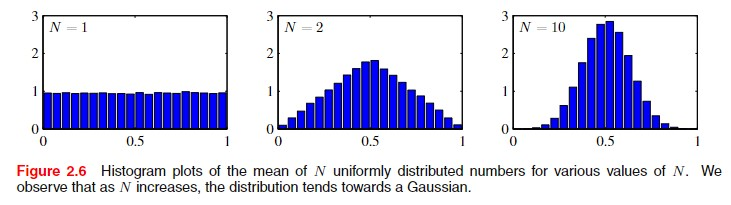
\includegraphics{bishop_26.jpg}
\end{figure}
\par
\textbf{Solução:}

De forma a atender a este exercício foi implementado em python um programa que verifica experimentalmente o Teorema Central do Limite (TCL) ao plotar histogramas das médias de variáveis aleatórias iid (independentemente e identicamente distribuídas) para dois tipos de distribuições: Uniforme(0,1) e Bernoulli($\mu$). O TCL afirma que, para um número suficientemente grande de variáveis aleatórias iid, a distribuição da média dessas variáveis tende a uma distribuição normal (Gaussiana), independentemente da forma da distribuição original. O código define três valores de $N$ (1, 2 e 10) e gera um número elevado de amostras $(num\_samples = 10000)$ para cada valor de N. Para cada conjunto de amostras, calcula-se a média e, em seguida, os histogramas dessas médias são plotados. No caso da distribuição Uniforme$(0,1)$, amostras são geradas com valores uniformemente distribuídos entre 0 e 1. No caso da distribuição de Bernoulli, amostras são geradas com probabilidade $\mu=0.7$. Os resultados podem ser observados na figura abaixo.

\begin{figure}[H]
    \caption{\textbf{Plot do resultado}}
       \centering
       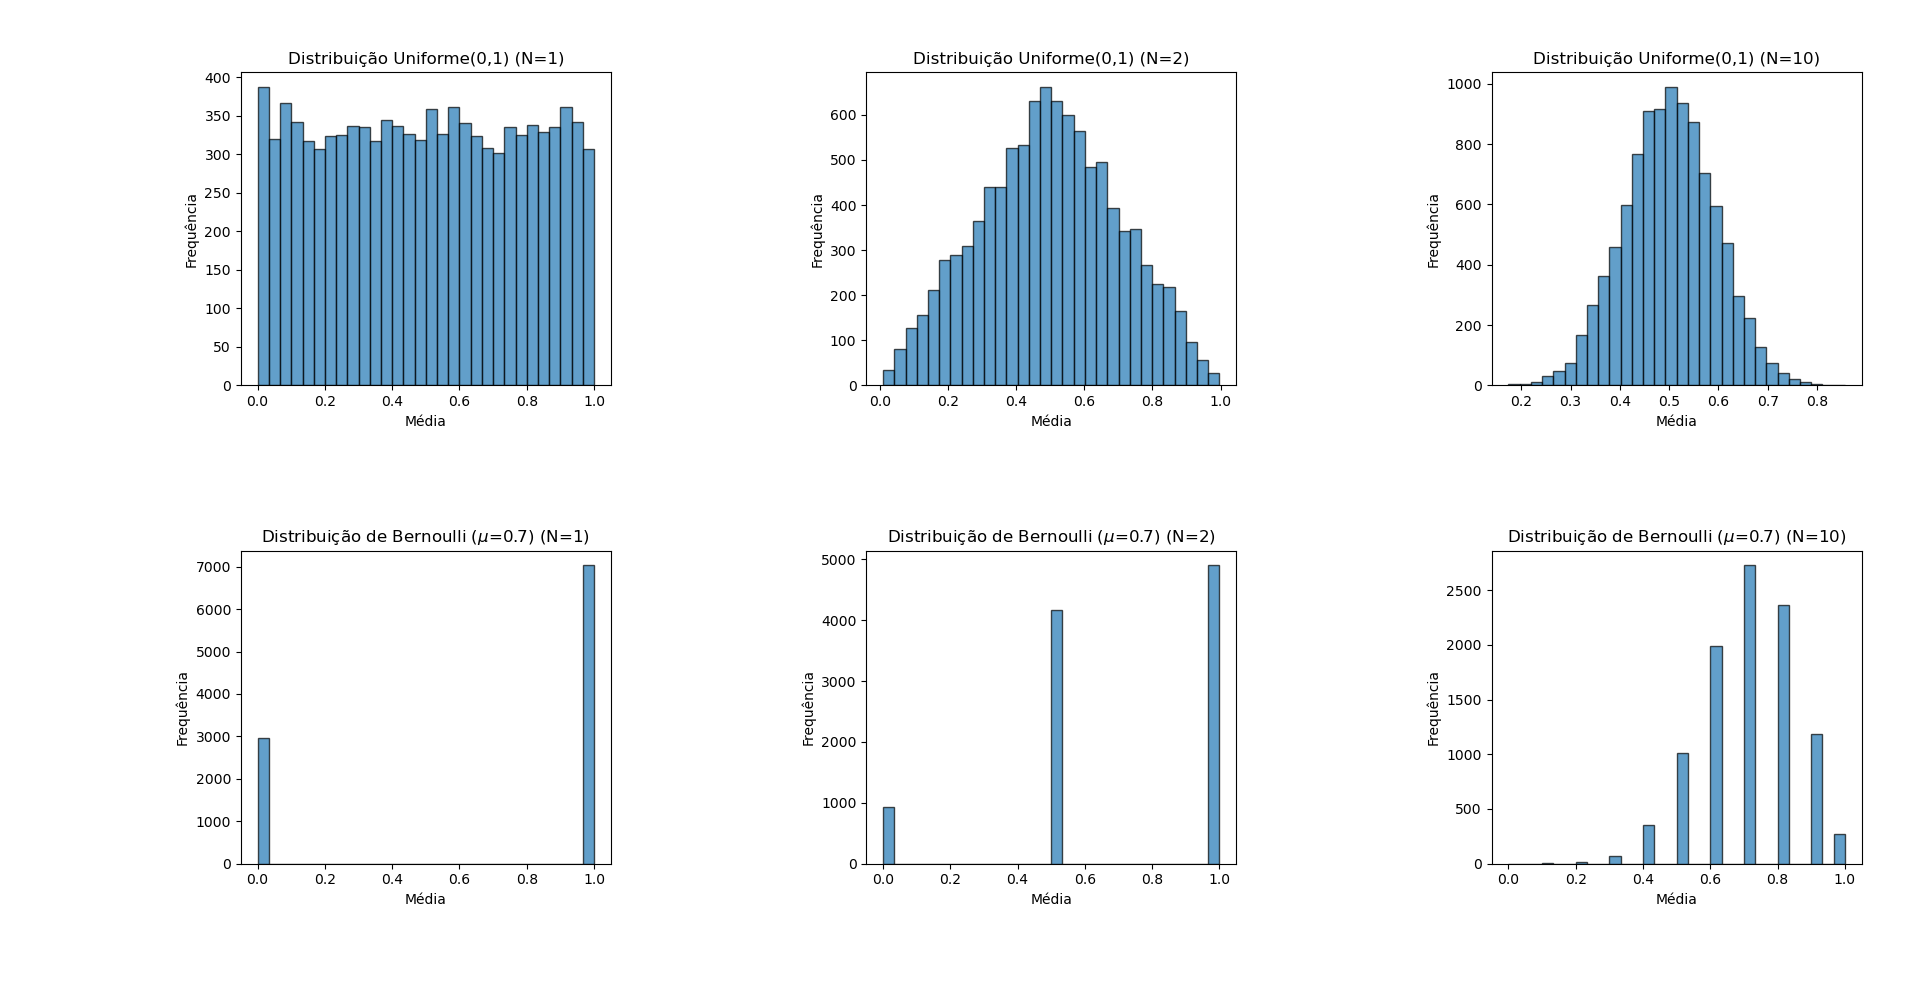
\includegraphics[width=\textwidth]{ex2.png}
\end{figure}

Os resultados mostram que, para $N$ pequeno ($N=1$ ou $N=2$), as distribuições das médias ainda refletem a forma original das distribuições de amostra. No entanto, conforme $N$ aumenta para 10, as distribuições das médias começam a se aproximar de uma forma mais simétrica e similar à curva normal, confirmando a previsão do TCL. Este comportamento é mais evidente na distribuição Uniforme(0,1), onde a média das amostras se torna claramente gaussiana. Na distribuição de Bernoulli, o efeito é semelhante, mas a convergência é influenciada pela natureza da distribuição original $(\mu=0.7)$. Essas observações confirmam que, à medida que o tamanho da amostra $N$ aumenta, a distribuição das médias converge para uma distribuição normal, conforme previsto pelo Teorema Central do Limite.


%%%%%%%%%%%%%%%%%%%%%%%%%%%%%%%%%%%%%%%%%%%%%%%%%%%%%%%%%%%%%%%

\item \textbf{Verificação experimental da Law of Large Numbers - LLN} \par
Considere N variáveis aleatórias independentes geradas a partir de uma distribuição normal padrão (isto é, Gaussiana de média 0 e variância 1). Compute o estimador média amostral. Repita o experimento diversas vezes e plote o histograma desse estimador para um dado valor de N. Mostre que, conforme N aumenta, o histograma desse estimador fica cada vez mais estreito em torno do valor correto (i.e., variância vai diminuindo), que é zero.
\par
\textbf{Solução:}

De forma a atender a este exercício foi implementado em python um programa que utiliza o conceito da Lei dos Grandes Números para ilustrar como a média amostral de variáveis aleatórias independentes e identicamente distribuídas (i.i.d.) converge para a média da população conforme o tamanho da amostra ($N$) aumenta. A Lei dos Grandes Números afirma que, à medida que o número de amostras aumenta, a média amostral se aproxima da média esperada da distribuição. No caso deste código, ele gera $N$ variáveis aleatórias a partir de uma distribuição normal padrão (com média 0 e variância 1), calcula a média dessas variáveis e repete esse processo 10.000 vezes para diferentes valores de $N$. Os histogramas das médias amostrais são então plotados para valores crescentes de $N$, demonstrando que, conforme $N$ aumenta, a variabilidade (ou seja, a largura) das médias amostrais diminui e se concentra em torno de zero, a média real da distribuição. Os resultados podem ser observados na figura abaixo.

\begin{figure}[H]
    \caption{\textbf{Plot do resultado}}
       \centering
       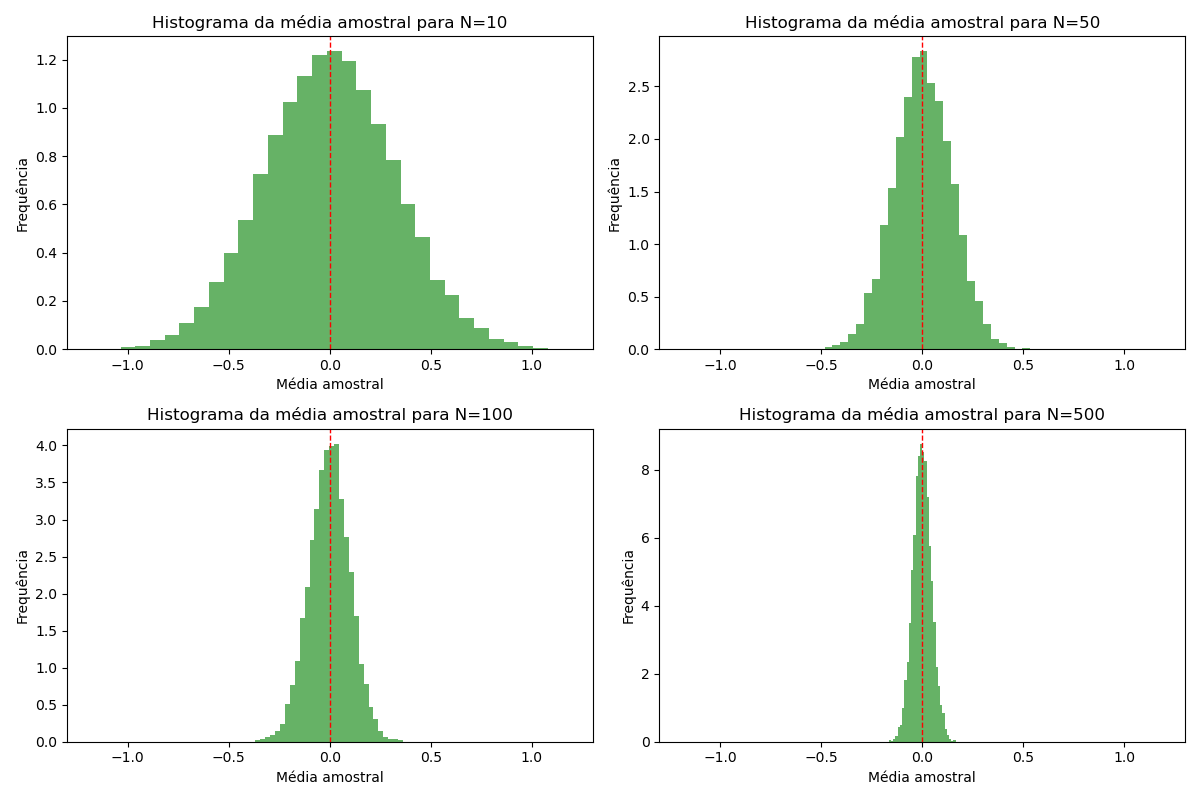
\includegraphics[width=\textwidth]{ex3.png}
\end{figure}


Pelos resultados, observamos que os histogramas das médias amostrais se tornam progressivamente mais estreitos à medida que o valor de $N$ aumenta. Para $N = 10$, o histograma é relativamente largo, indicando uma maior variação nas médias amostrais. Para $N = 50$ e $N = 100$, o histograma se torna mais concentrado em torno de zero, e para $N = 500$, o histograma é ainda mais estreito. Isso confirma empiricamente a Lei dos Grandes Números, mostrando que a variância da média amostral diminui à medida que o tamanho da amostra aumenta, resultando em uma estimativa mais precisa da média da população. Assim, o experimento visualmente demonstra como a média amostral converge para o valor esperado, reforçando a compreensão teórica desse importante conceito estatístico.



%%%%%%%%%%%%%%%%%%%%%%%%%%%%%%%%%%%%%%%%%%%%%%%%%%%%%%%%%%%%%%%

\item \textbf{Estimação de pdf} \par
Tente replicar os resultados exibidos nas figuras 2.24 e 2.25 do livro. Para isso, gere uma amostra de N=50 dados cuja distribuição é dada pela curva em verde (corresponde a uma mistura de 2 gaussianas - veja equação 
$$p(x) = \sum_{k=1}^{K}\pi_k \mathcal{N} (x|\mu_k. \Sigma_k)$$ 
e escolha os parâmetros dessa distribuição da forma que quiser). Estime a pdf do modelo gerador dos dados utilizando 2 métodos: histograma e kernel Gaussiano. Para o parâmetro h, utilize os mesmos valores das figuras.
\begin{figure}[H]
    \caption{\textbf{Figura 2.24 do Bishop}}
       \centering
       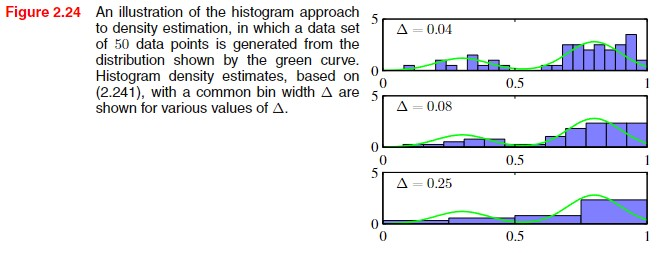
\includegraphics{bishop_224.jpg}
\end{figure}
\begin{figure}[H]
    \caption{\textbf{Figura 2.25 do Bishop}}
       \centering
       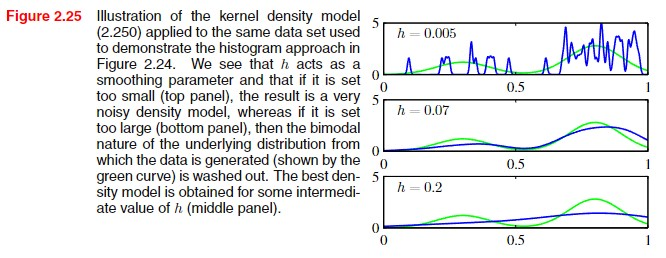
\includegraphics{bishop_225.jpg}
\end{figure}
\par
\textbf{Solução:}

O código python implementado resolver esse exercício realiza a estimação da função de densidade de probabilidade (pdf) de um modelo gerador de dados que segue uma distribuição representada por uma mistura de duas gaussianas. Inicialmente, são definidos os parâmetros das duas distribuições gaussianas, como média ($\mu$), desvio padrão ($\sigma$) e peso ($\pi$) de cada componente da mistura. Em seguida, é gerada uma amostra de dados com base nessas distribuições.

Para estimar a pdf do modelo gerador, são utilizados dois métodos: histograma e kernel Gaussiano. No método do histograma, a amostra de dados é dividida em intervalos (bins) de largura determinada por diferentes valores de $\Delta$, e a densidade é estimada calculando a frequência relativa de dados em cada bin. No método do kernel Gaussiano, é ajustada uma função de densidade probabilística utilizando a técnica de Kernel Density Estimation (KDE) com diferentes larguras de banda ($h$). Os resultados podem ser observados na figura abaixo.

\begin{figure}[H]
    \caption{\textbf{Plot do resultado}}
       \centering
       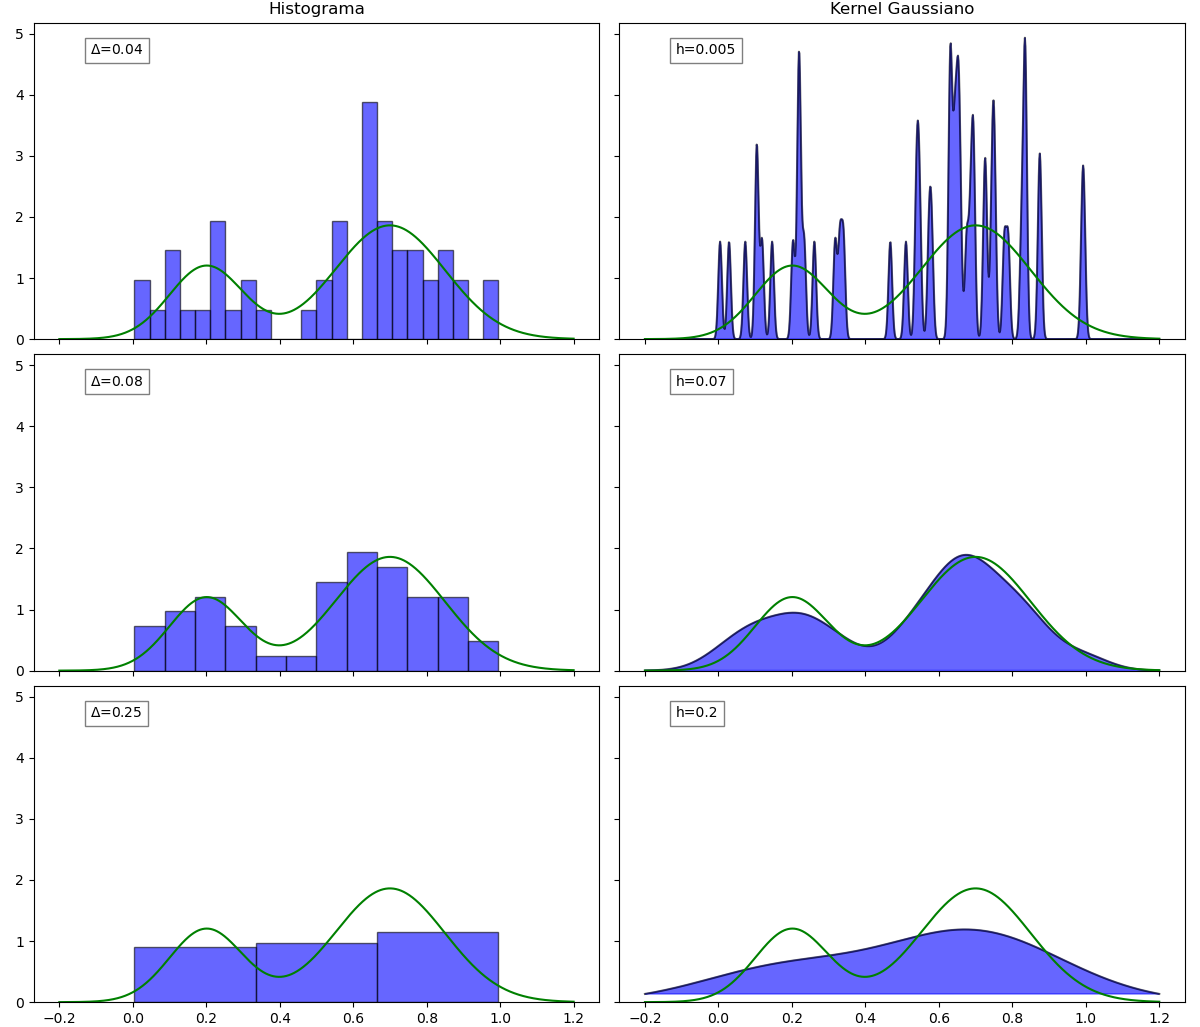
\includegraphics[width=\textwidth]{ex4.png}
\end{figure}

Na figura, é possível observar os resultados dos dois métodos de estimação de pdf para diferentes valores de $\Delta$ e $h$. No subplot da esquerda de cada linha, são plotados o histograma da amostra de dados (em azul) e a curva do modelo gerador (em verde). No subplot da direita, são mostradas as curvas de densidade estimadas pelo kernel Gaussiano (em preto, com sombra azul) sobrepostas à curva do modelo gerador (em verde). Além disso, são exibidos os valores de delta e largura de banda utilizados em cada subplot.

Em relação aos resultados, pode-se observar que a estimação da pdf pelo kernel Gaussiano tende a suavizar a distribuição em comparação com o método do histograma, especialmente quando a largura de banda ($h$) é maior. Isso ocorre porque o kernel Gaussiano utiliza uma abordagem mais suave e contínua para estimar a densidade, enquanto o histograma é mais sensível à escolha dos bins e pode apresentar variações bruscas na representação da distribuição, especialmente com valores pequenos de $\Delta$.


%%%%%%%%%%%%%%%%%%%%%%%%%%%%%%%%%%%%%%%%%%%%%%%%%%%%%%%%%%%%%%%

\item \textbf{Classificador K-NN} \par
Considere 2 classes, C1 e C2, que correspondem aos seguintes modelos geradores: 

C1: pdf Gaussiana de média -1 e variância 1

C2: pdf Gaussiana de média 1 e variância 1

Gere 10 observações de cada uma dessas classes e assuma que você sabe exatamente a classe de cada um dos 20 pontos gerados (10 pontos para cada classe). Em seguida, gere mais 2 observações de cada classe e assuma que você NÃO sabe de qual classe esses novos dados pertencem. Utilize a técnica de K-NN, considerando diferentes valores de K, para classificar os 4 novos dados.

OBS: Plote os resultados utilizando cores e símbolos para facilitar a interpretação. Por exemplo: Para os 20 pontos conhecidos, represente-os usando `bolinhas' vermelhas para C1 e azuis para C2. Para os 4 pontos a serem classificados, mantenha o código de cores (para sabermos identificar qual era a classe correta) e use novos símbolos para identificar se a classificação foi correta (use um `quadrado') ou se a classificação foi errada (neste caso, use um `x').

Se for usar outros símbolos e cores, não tem problema. Só não esqueça de fazer uma
legenda ou caption que me permita compreender a figura.


\par
\textbf{Solução:}

O código realiza um experimento utilizando o Classificador K-Vizinhos Mais Próximos (K-NN) para classificar dados gerados a partir de duas distribuições Gaussianas diferentes, representando duas classes, C1 e C2. Inicialmente, são gerados 10 pontos para cada classe, conhecidos, e mais 2 pontos de cada classe, inicialmente desconhecidos. O K-NN é aplicado considerando diferentes valores de K (1, 3, 5, 7) para classificar os 4 novos pontos. O K-NN funciona encontrando os K vizinhos mais próximos de um ponto desconhecido e atribuindo a ele a classe mais comum entre esses vizinhos. No código, a classe KNeighborsClassifier é usada para treinar o modelo com os dados conhecidos e prever a classe dos novos pontos. No gráfico resultante, os pontos conhecidos são representados por bolinhas vermelhas (C1) e azuis (C2), enquanto os pontos classificados corretamente recebem um quadrado da mesma cor da classe e os classificados incorretamente recebem um "x" da cor que foram incorretamente classificados. Esse método ilustra como o K-NN pode ser usado para classificar novos dados com base em dados conhecidos, sendo sensível ao número de vizinhos considerados. Os resultados podem ser observados na figura abaixo.

\begin{figure}[H]
    \caption{\textbf{Plot do resultado}}
       \centering
       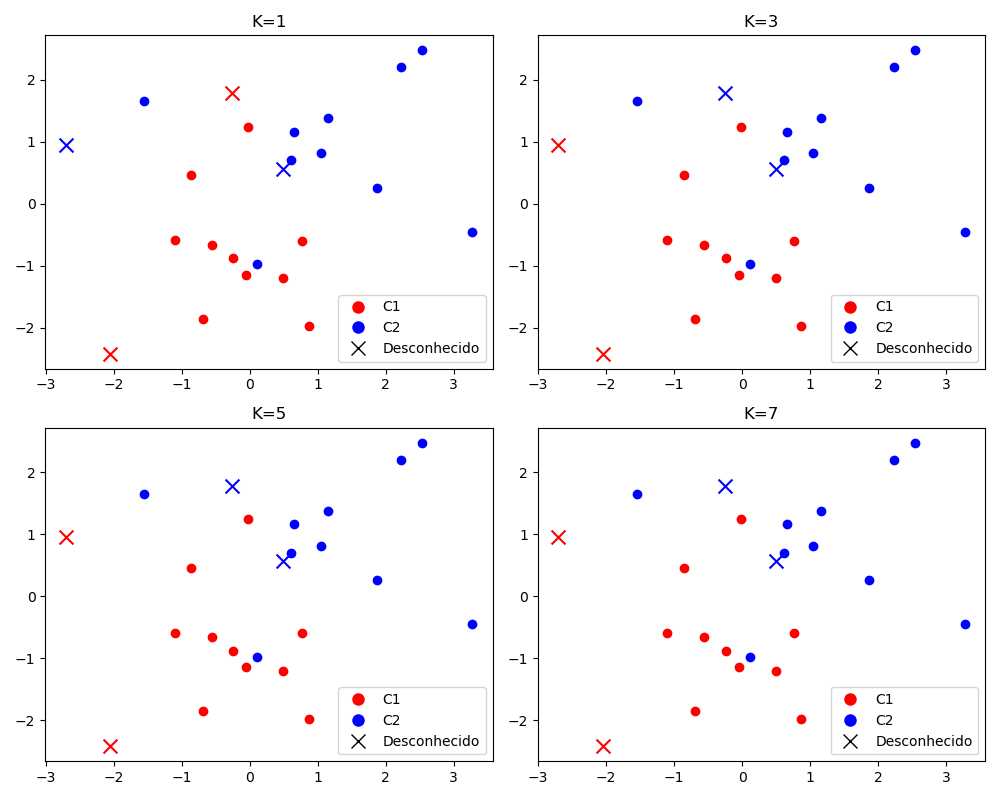
\includegraphics[width=\textwidth]{ex5.png}
\end{figure}


Podemos observar que a classificação dos pontos desconhecidos varia conforme o valor de K. Com K=1, o modelo tende a se ajustar demais aos dados conhecidos, resultando em uma classificação sensível a outliers. Com K=3, 5 e 7, o modelo suaviza essa sensibilidade, e a classificação dos pontos desconhecidos tende a ser mais estável. No entanto, é importante notar que a escolha ideal de K depende do contexto e da natureza dos dados, buscando um equilíbrio entre o viés e a variância do modelo para obter a melhor generalização possível.


%%%%%%%%%%%%%%%%%%%%%%%%%%%%%%%%%%%%%%%%%%%%%%%%%%%%%%%%%%%%%%%



\end{enumerate}